\subsection{Descripción general de la solución}

Una vez relevados todos los requerimientos asociados al proyecto y revisados los diseños del prototipo anterior del SAL/T, se generó un diagrama en bloques de la solución donde se contemplan todos los módulos involucrados, que se puede visualizar en la figura \ref{fig:diagrama_bloques}. Se observa que el sistema interactúa con distintos elementos externos pertenecientes a la formación ferroviaria, como los sistemas instrumentados de seguridad o el control central de la formación. Se considera también el uso de una fuente externa que permite alimentar al SAL/T con 5 V de tensión continua generados a partir de las baterías de alimentación de los trenes que están en un rango de entre 72-110 VDC dependiendo del modelo de la formación. También existe una interacción con el bus de datos que conecta el registrador de eventos Hasler Teloc 1500 \cite{hasler} con el indicador de velocidad Hasler y otra interacción con un subsistema externo que realiza la interpretación de la velocidad a partir de la señal generada por un generador de impulsos; ambas interactúan con las interfaces RS-485 del sistema. \\


Con el diagrama en bloques del sistema, se pueden considerar las distintas interacciones que va a tener el controlador principal y elegir algún microcontrolador (MCU) que tenga las interfaces necesarias para conectarse con todos los módulos, y la capacidad de procesamiento adecuada para este tipo de aplicaciones. Después de analizar las distintas alternativas disponibles en el mercado, se eligió el microcontrolador STM32F429ZI ya que tiene un buen rendimiento por su core ARM Cortex-M4 que corre en una frecuencia de hasta 180 MHz con una unidad de punto flotante, soporta múltiples interfaces de comunicación (I2C, SPI, UART, GPIO, ADC, etc.) y cuenta con memoria flash y RAM suficientes para un firmware complejo. Otra ventaja de usar los microcontroladores de ST es que cuentan con el entorno de desarrollo STM32CubeIDE que es muy amigable para la programación del MCU y la configuración de todos los periféricos. \\ 


Una vez seleccionado el microcontrolador principal, se decidió armar el prototipo del SAL/T a partir de una placa de desarrollo que contiene al STM32F429ZI para mantener el alcance del proyecto dentro de lo esperado para este trabajo. Por lo tanto, se seleccionó la placa de desarrollo NUCLEO F429ZI que contiene el MCU mencionado. Esta placa incluye una interfaz ST-LINK/V2-1 que permite la programación y \textit{debugging} del microcontrolador sin necesidad de hardware adicional. También trae circuitos adicionales como el oscilador de cristal, circuito de reset, LEDs, botones de prueba y reguladores de tensión que permiten alimentar la placa con distintos niveles de tensión. Todas estas características facilitan el desarrollo del proyecto porque permiten probar algunos circuitos, partes del firmware y la comunicación con otros módulos, sin tener todavía fabricado un PCB diseñado ad hoc para el proyecto. \\


Con la placa de desarrollo definida como base del sistema, se realizó una búsqueda de los posibles circuitos o módulos para implementar los distintos bloques que cumplan con los requerimientos acordados y que permitan hacer un uso distribuido de las interfaces que ofrece el MCU. Para la selección de componentes y módulos, se consideraron algunos criterios que facilitan la selección. Por ejemplo, se intentó reutilizar módulos o componentes ya utilizados en otros proyectos del grupo GICSAFe para poder ayudarse de diseños y experiencias de uso previas; esto reduce la posibilidad de error o mal funcionamiento de los circuitos y acelera tiempos de descubrimiento en fallas ocultas que pueden traer asociadas. Otro criterio importante fue utilizar dos distribuidores de componentes electrónicos grandes (Mouser \cite{mouser} y Digikey \cite{digikey}) para verificar que estas partes estén disponibles y en stock de manera general y que sean recomendados para nuevos diseños y no en un estado cercano al final de su ciclo de vida (EOL, \textit{End-of-Life}); de esta manera se asegura que el prototipo y su implementación sean reproducibles y sus partes fáciles de conseguir en el mediano plazo. \\

Con una idea más clara de los circuitos que se podían usar para implementar los distintos bloques y sus variantes de comunicación con el MCU, se realizó el diagrama de la figura \ref{fig:diagrama_bloques_coms} que muestra los protocolos de comunicación entre el MCU y los distintos circuitos del sistema. Esto permitió hacer una asignación de las interfaces disponibles para cada bloque. 

\begin{figure}[H]
    \centering
    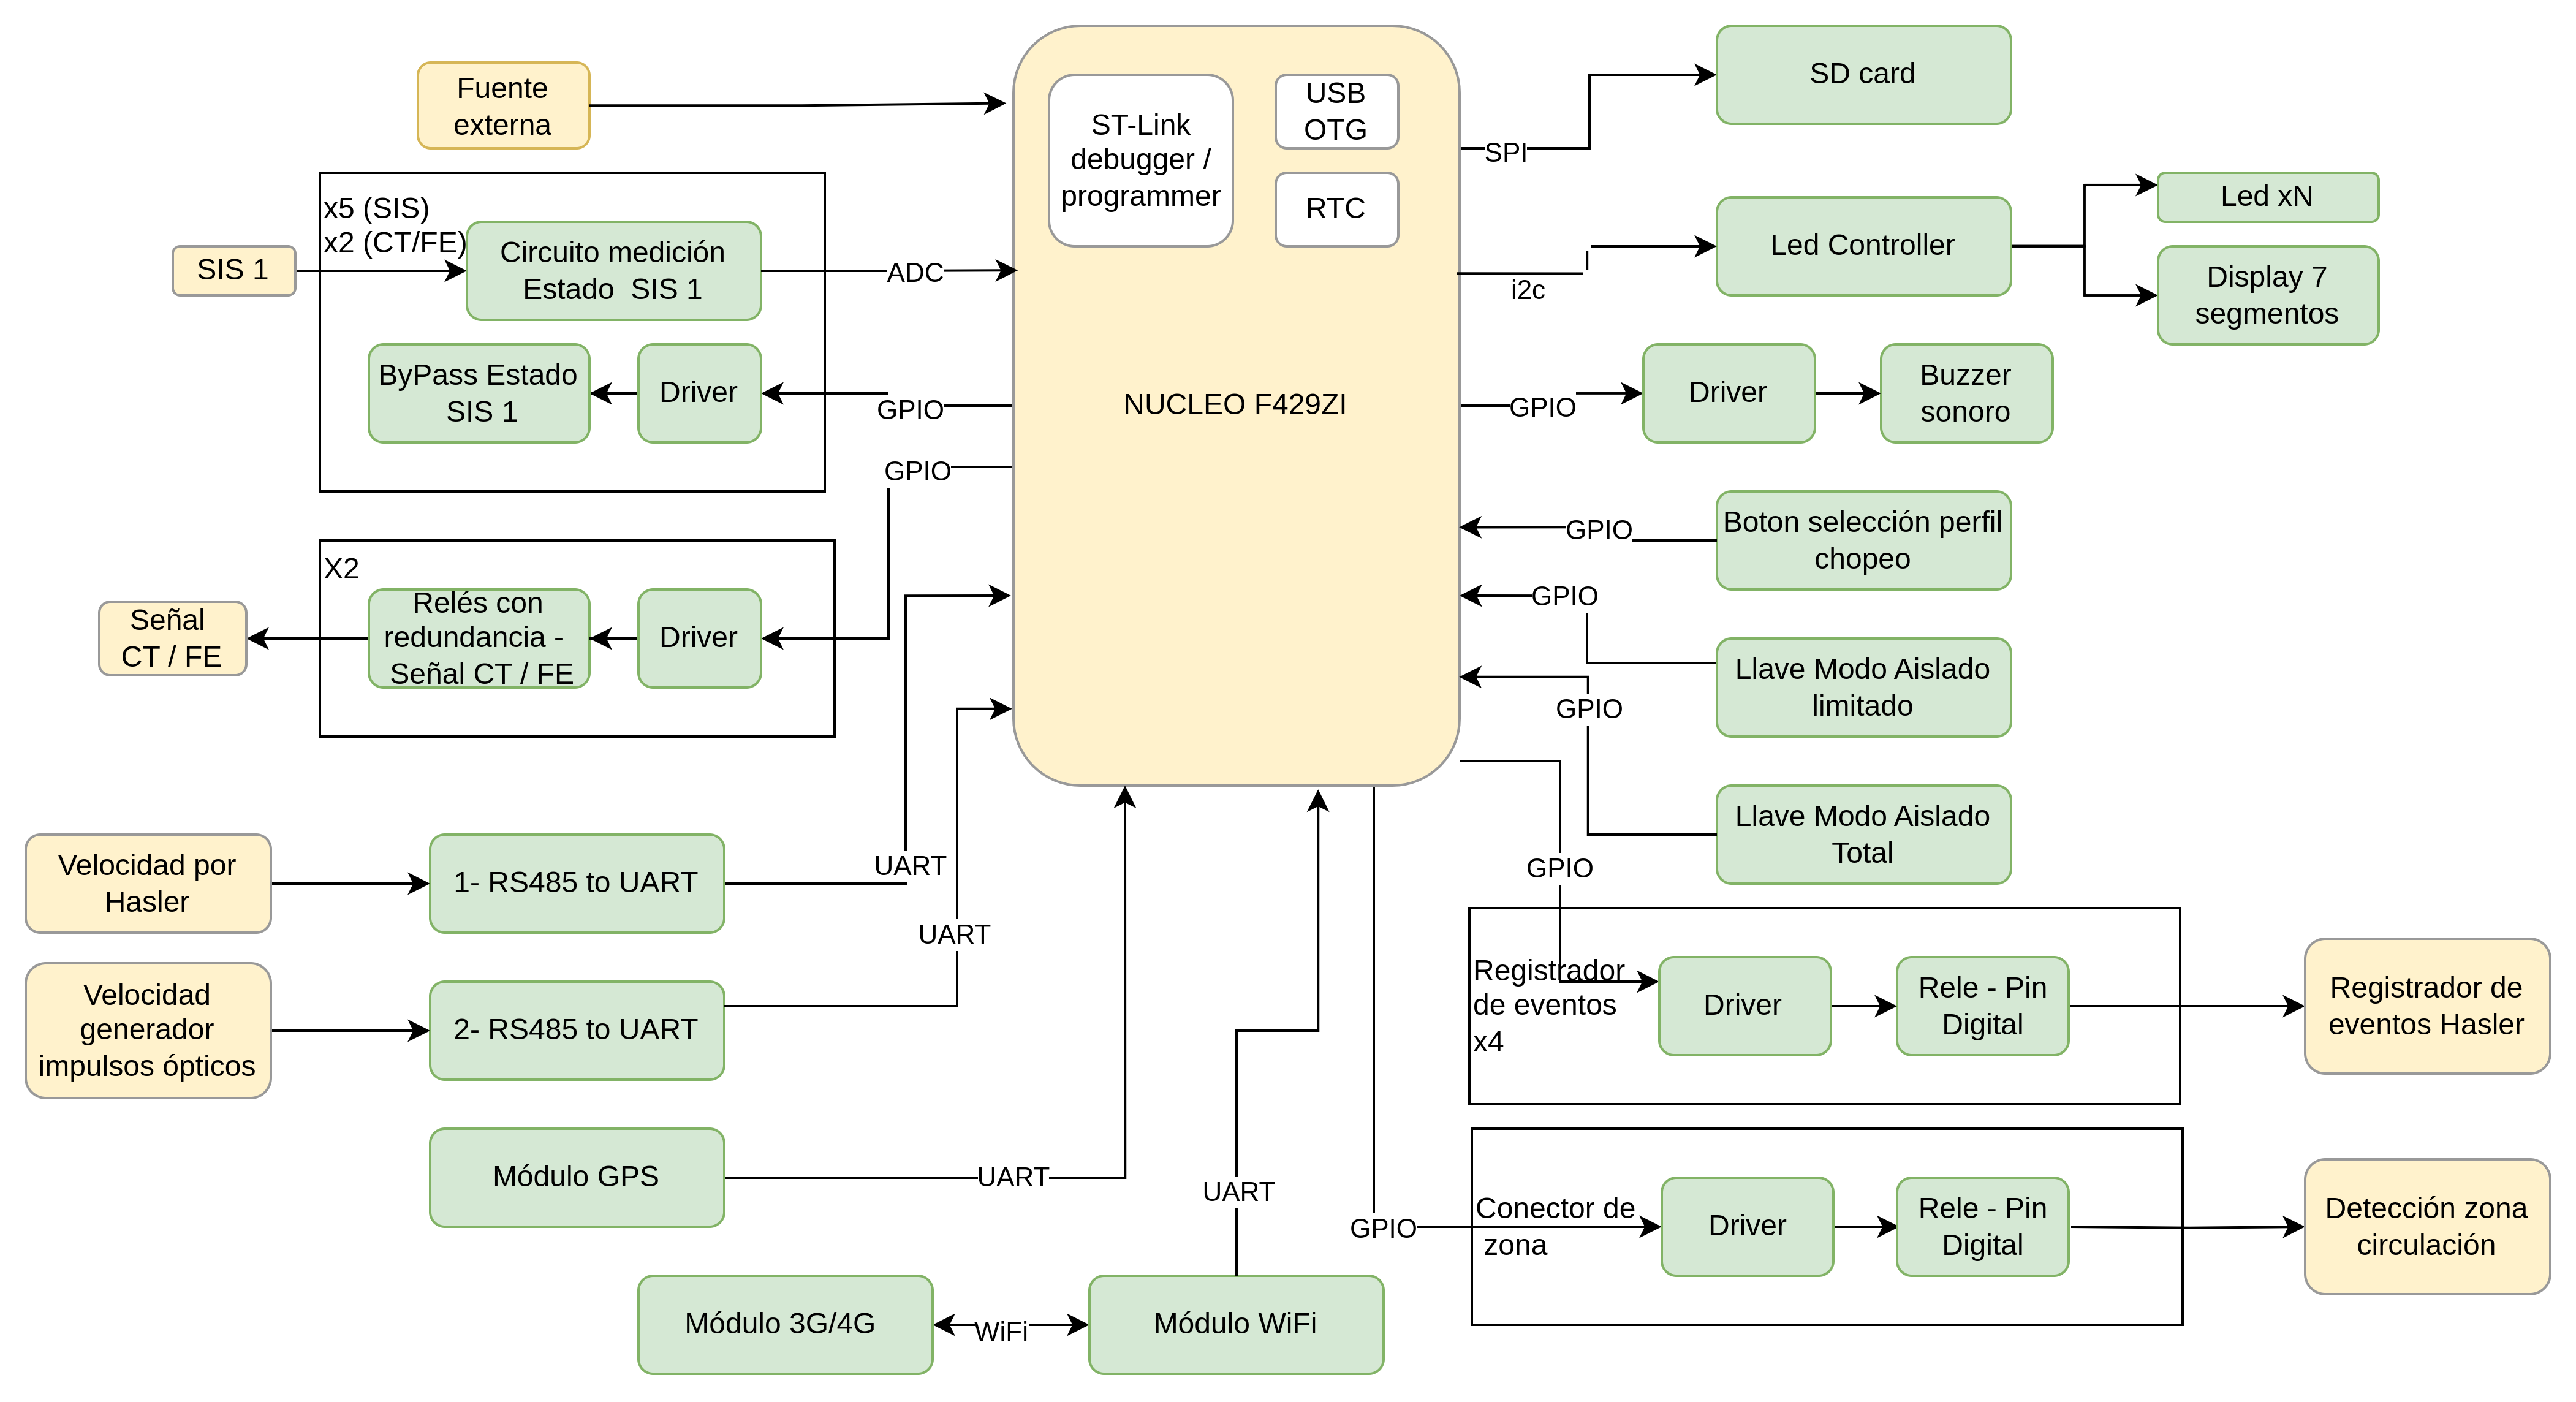
\includegraphics[width =  \linewidth]{img/diagrama_con_coms.png}
    \caption{Diagrama con interfaces de comunicación del SAL/T}
    \label{fig:diagrama_bloques_coms}
\end{figure}


Además, considerando que según los requisitos el sistema cuenta con un panel frontal para interactuar con el maquinista de la formación, se realizó el diseño de este panel para validar que tuviera todas las indicaciones e interacciones acordadas en los requerimientos. En la figura \ref{fig:panel_frontal} se puede visualizar la interfaz humano-máquina (IHM) que va a mostrar el estado del SAL/T en todo momento y permitir algunas interacciones mínimas al maquinista como la habilitación del modo aislado limitado o el cambio del perfil intermitente en caso de no contar con mediciones de velocidad activas. 
 
\begin{figure}[H]
    \centering
    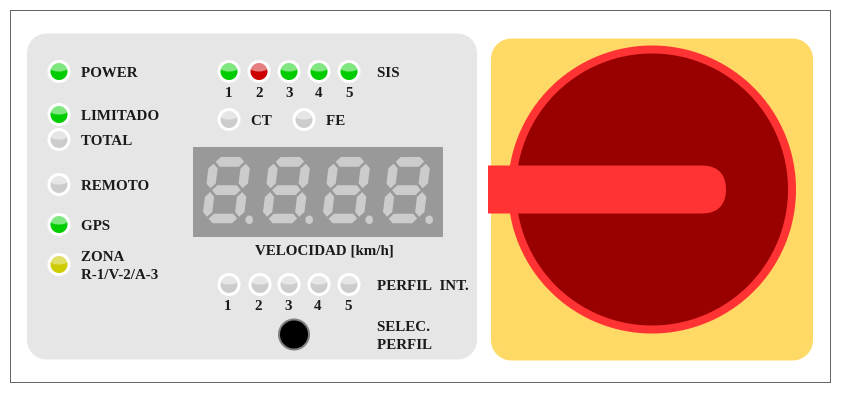
\includegraphics[width =  \linewidth]{img/ihm.png}
    \caption{Diseño del panel frontal del SAL/T}
    \label{fig:panel_frontal}
\end{figure}

Para comprender el diseño de los circuitos de medición y aislamiento de los SIS, así como la activación de las señales críticas de corte de tracción (CT) y freno de emergencia (FE), es importante entender cómo es la conexión en una formación ferroviaria entre los SIS y las señales críticas. Lo primero a considerar es que las líneas de activación de la señal CT y la de la señal FE son independientes; cada una tiene una electroválvula separada e interactúa con los SIS en una línea propia. Luego, para cada una de estas señales críticas, existe una conexión en serie entre la alimentación de la electroválvula, una llave cerrada que se abre en caso de falla del SIS para cada uno de los SIS, la electroválvula que habilita y deshabilita la señal crítica y tierra. Esta electroválvula, al seguir el concepto de \textit{fail-safe}, debe estar alimentada para poder liberar alguna de las señales críticas, y en caso de cortarse la alimentación, ya sea por una falla en la alimentación o porque uno de los SIS está fallando y reporta un estado inseguro abriendo la llave, se activa la señal de CT o de FE para frenar la formación. Este esquema se puede visualizar en la figura \ref{fig:lineas_ct_fe}.\\


\begin{figure}[H]
    \centering
    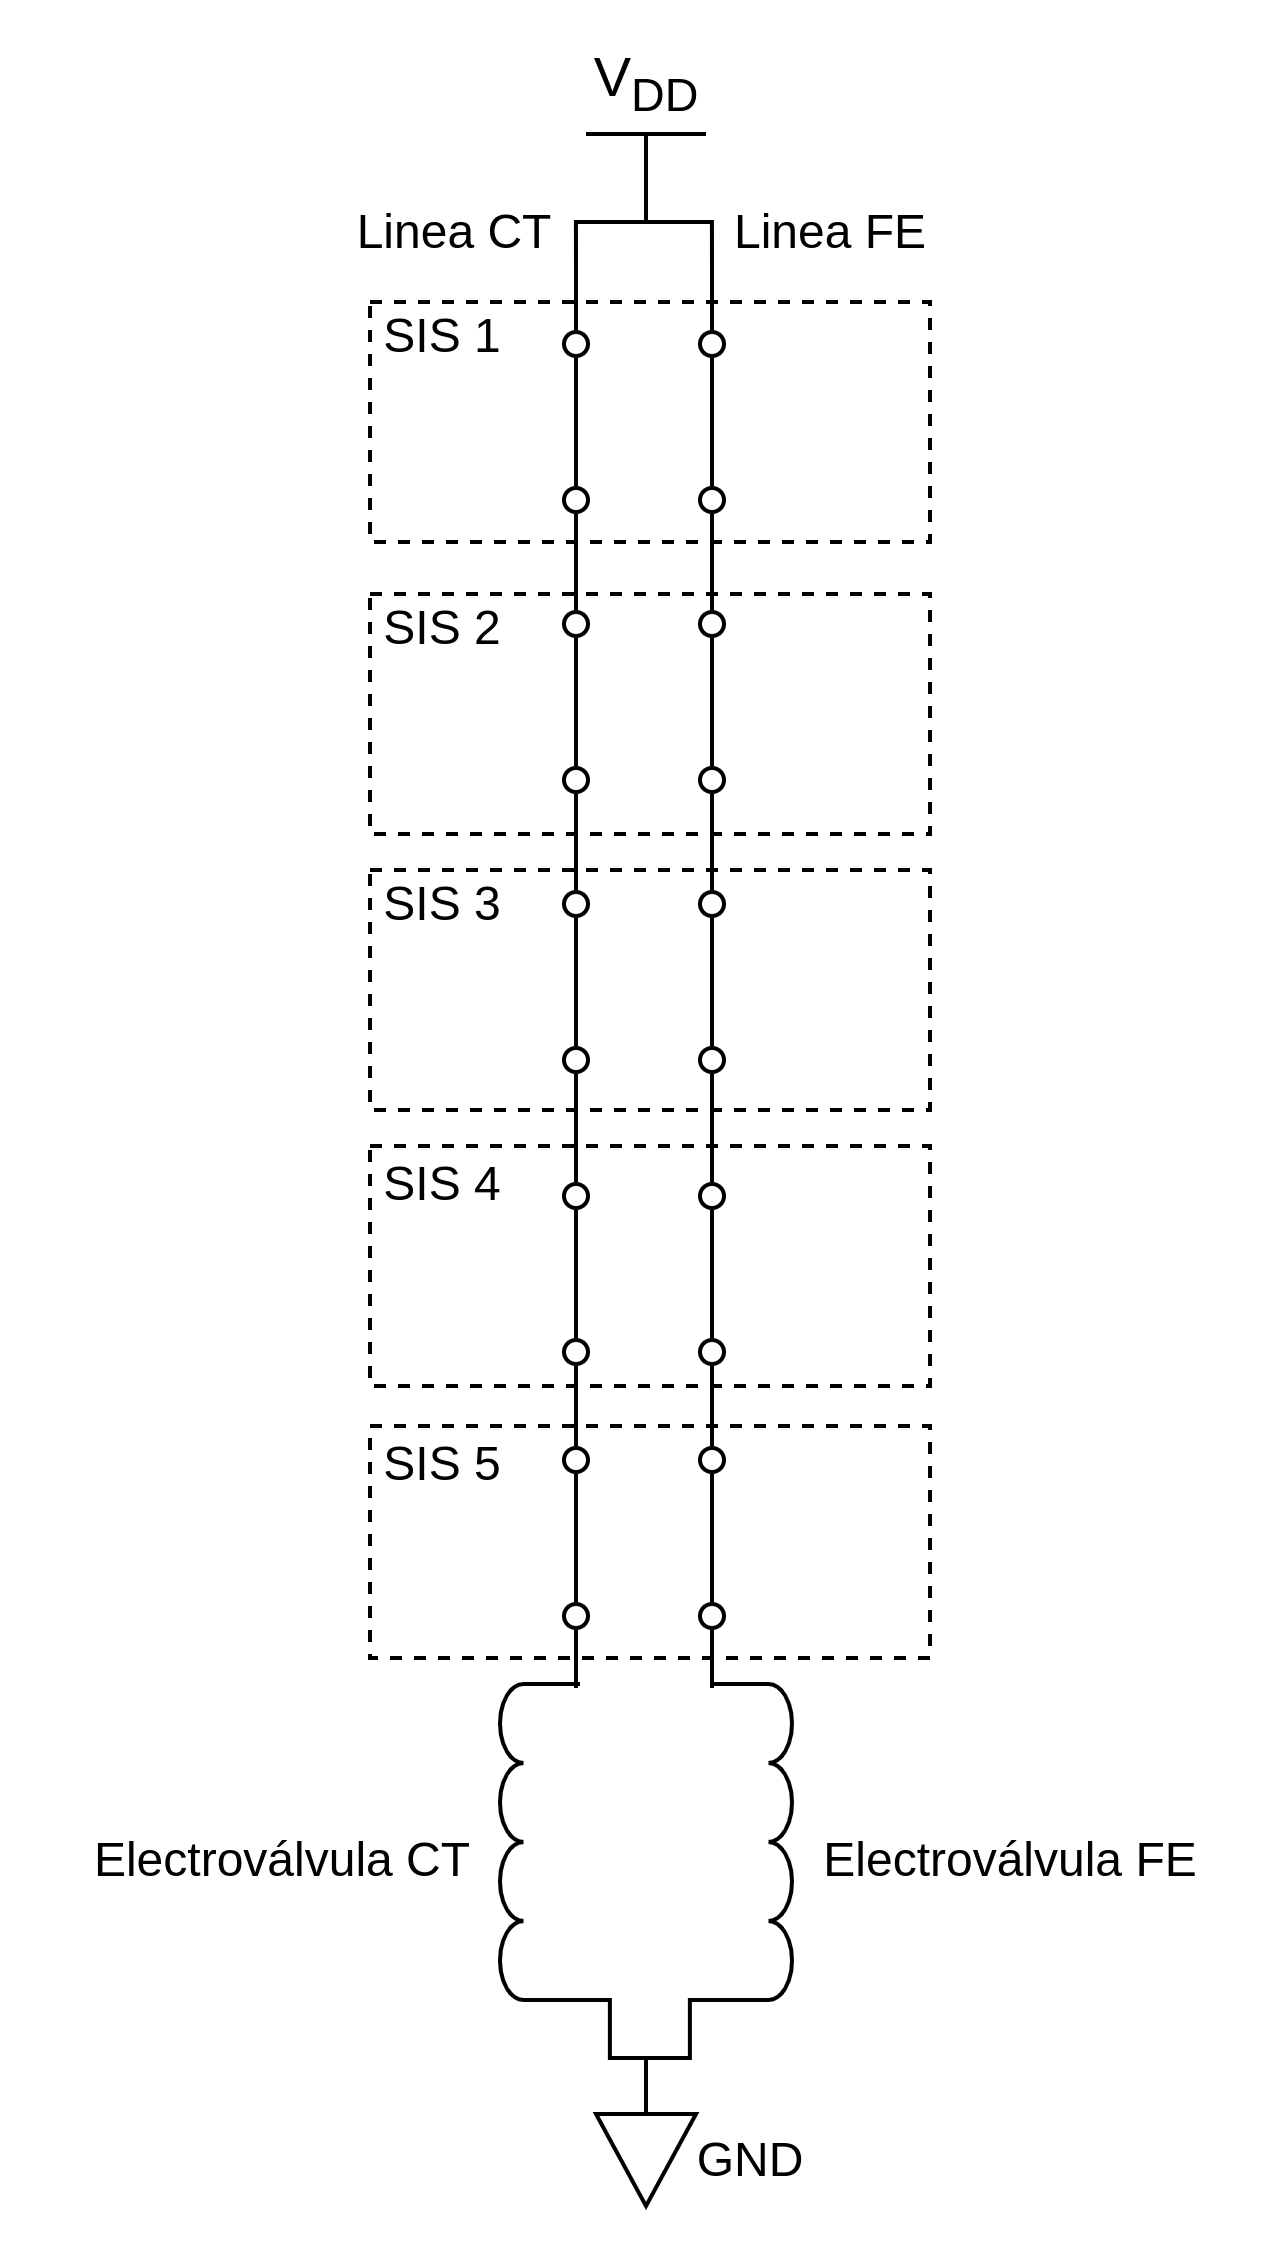
\includegraphics[width =  0.5\linewidth]{img/lineas_ct_fe.png}
    \caption{Lineas de señales de CT y FE}
    \label{fig:lineas_ct_fe}
\end{figure}


La idea del proyecto SAL/T es no modificar la arquitectura actual de los sistemas dentro de la formación, sino agregar algunos circuitos más para poder incrementar su seguridad sin necesidad de cambios en lo preexistente. Por esto, se propuso realizar las conexiones de la figura \ref{fig:señales_criticas} para poder realizar mediciones del estado de cada SIS independientemente, poder aislar cualquiera de ellos en caso de entrar en un modo aislado limitado, y también tener un último control para la activación de las señales críticas imponiendo una alimentación por fuera de la línea de los SIS. En la figura se muestran 2 SIS a modo de ejemplo y la línea de la señal de FE, pero el proyecto contempla 5 SIS y este mismo esquema para la señal de FE y CT. 


\begin{figure}[H]
    \centering
    \includegraphics[width = 0.8 \linewidth]{img/señales_criticas.jpeg}
    \caption{Diseño de conexión con SIS y señales críticas en el SAL/T}
    \label{fig:señales_criticas}
\end{figure}

Con la arquitectura general de la solución ya definida, se decidió modularizar el sistema en dos placas separadas. Una placa principal donde se va a realizar todo el procesamiento del sistema, se van a recibir las mediciones de velocidad, del estado de los SIS, de la posición, los comandos remotos y donde se va a interactuar con el aislamiento de los SIS, la activación de las señales críticas, el registro de eventos internos y externos de manera local y remoto y la descarga de los eventos guardados. La segunda placa va a estar dedicada a la interacción con el maquinista y va a contar con el panel frontal, los LEDs indicativos, el display para mostrar la velocidad de la formación y un botón para seleccionar el perfil intermitente a ejecutar en el modo aislado limitado cuando no se cuenta con mediciones de velocidad válidas. De esta manera, se permite mayor flexibilidad en el diseño de las placas y una mejor modularización del sistema. \\ 

Para realizar el diseño del hardware se utilizó KiCad \cite{kicad} versión 6; una herramienta de software libre utilizada para el diseño de esquemáticos y PCB. También se utilizó LTspice \cite{LTspice}; un simulador de circuitos de código abierto desarrollado por Analog Devices, utilizado para simular el comportamiento de los distintos circuitos en la etapa de diseño. Para llevar un control de versiones, tanto de los archivos de diseño de hardware como de firmware, se utilizó GitHub \cite{github}; una plataforma de desarrollo colaborativo que utiliza Git \cite{git} como sistema de control de versiones que permite almacenar, gestionar y rastrear cambios en el código fuente de sus proyectos. Se utilizó un repositorio donde se fueron avanzando los distintos módulos (tanto de hardware como de firmware) del proyecto en distintas \textit{branches} para finalmente llegar a una versión unificada en la \textit{branch} principal. El repositorio es público y accesible en \href{https://github.com/martinanus/salt}{\textit{github.com/martinanus/salt}} \cite{repo}.






